\chapter{Long Lived Particles}

This chapter presents some context and basic information about searches for \acp{LLP}. 

\section{Basics}

Any particle's lifetime is given as the inverse of its \emph{width}:

\begin{equation}
\tau = \frac{1}{\Gamma}
\end{equation}

Where its width can be defined as:

\begin{equation}
\Gamma = \frac{1}{2m_{X}} \int d\Pi_f \big| \mathcal{M}(m_X \rightarrow \{p_f\})\big|^2
\end{equation}

where $m_X$ is the mass of the particle, $mathcal{M}$ is the matrix element for the particle's decay into its decay products $\{p_f\}$ and $d\Pi_f$ is the Lorentz-invariant phase space of the decay. 

In order for the lifetime of a particle to be long, the width must be small, meaning that the matrix element or allowed phase space must be small. A small matrix element can be caused by a small coupling, and a small phase space can be caused by almost-degenerate mass spectra or very offshel intermediate states. All of which are common in both the \ac{SM} and many \ac{BSM} theories. 




\section{In Context}

\begin{figure}[htbp]
\centering
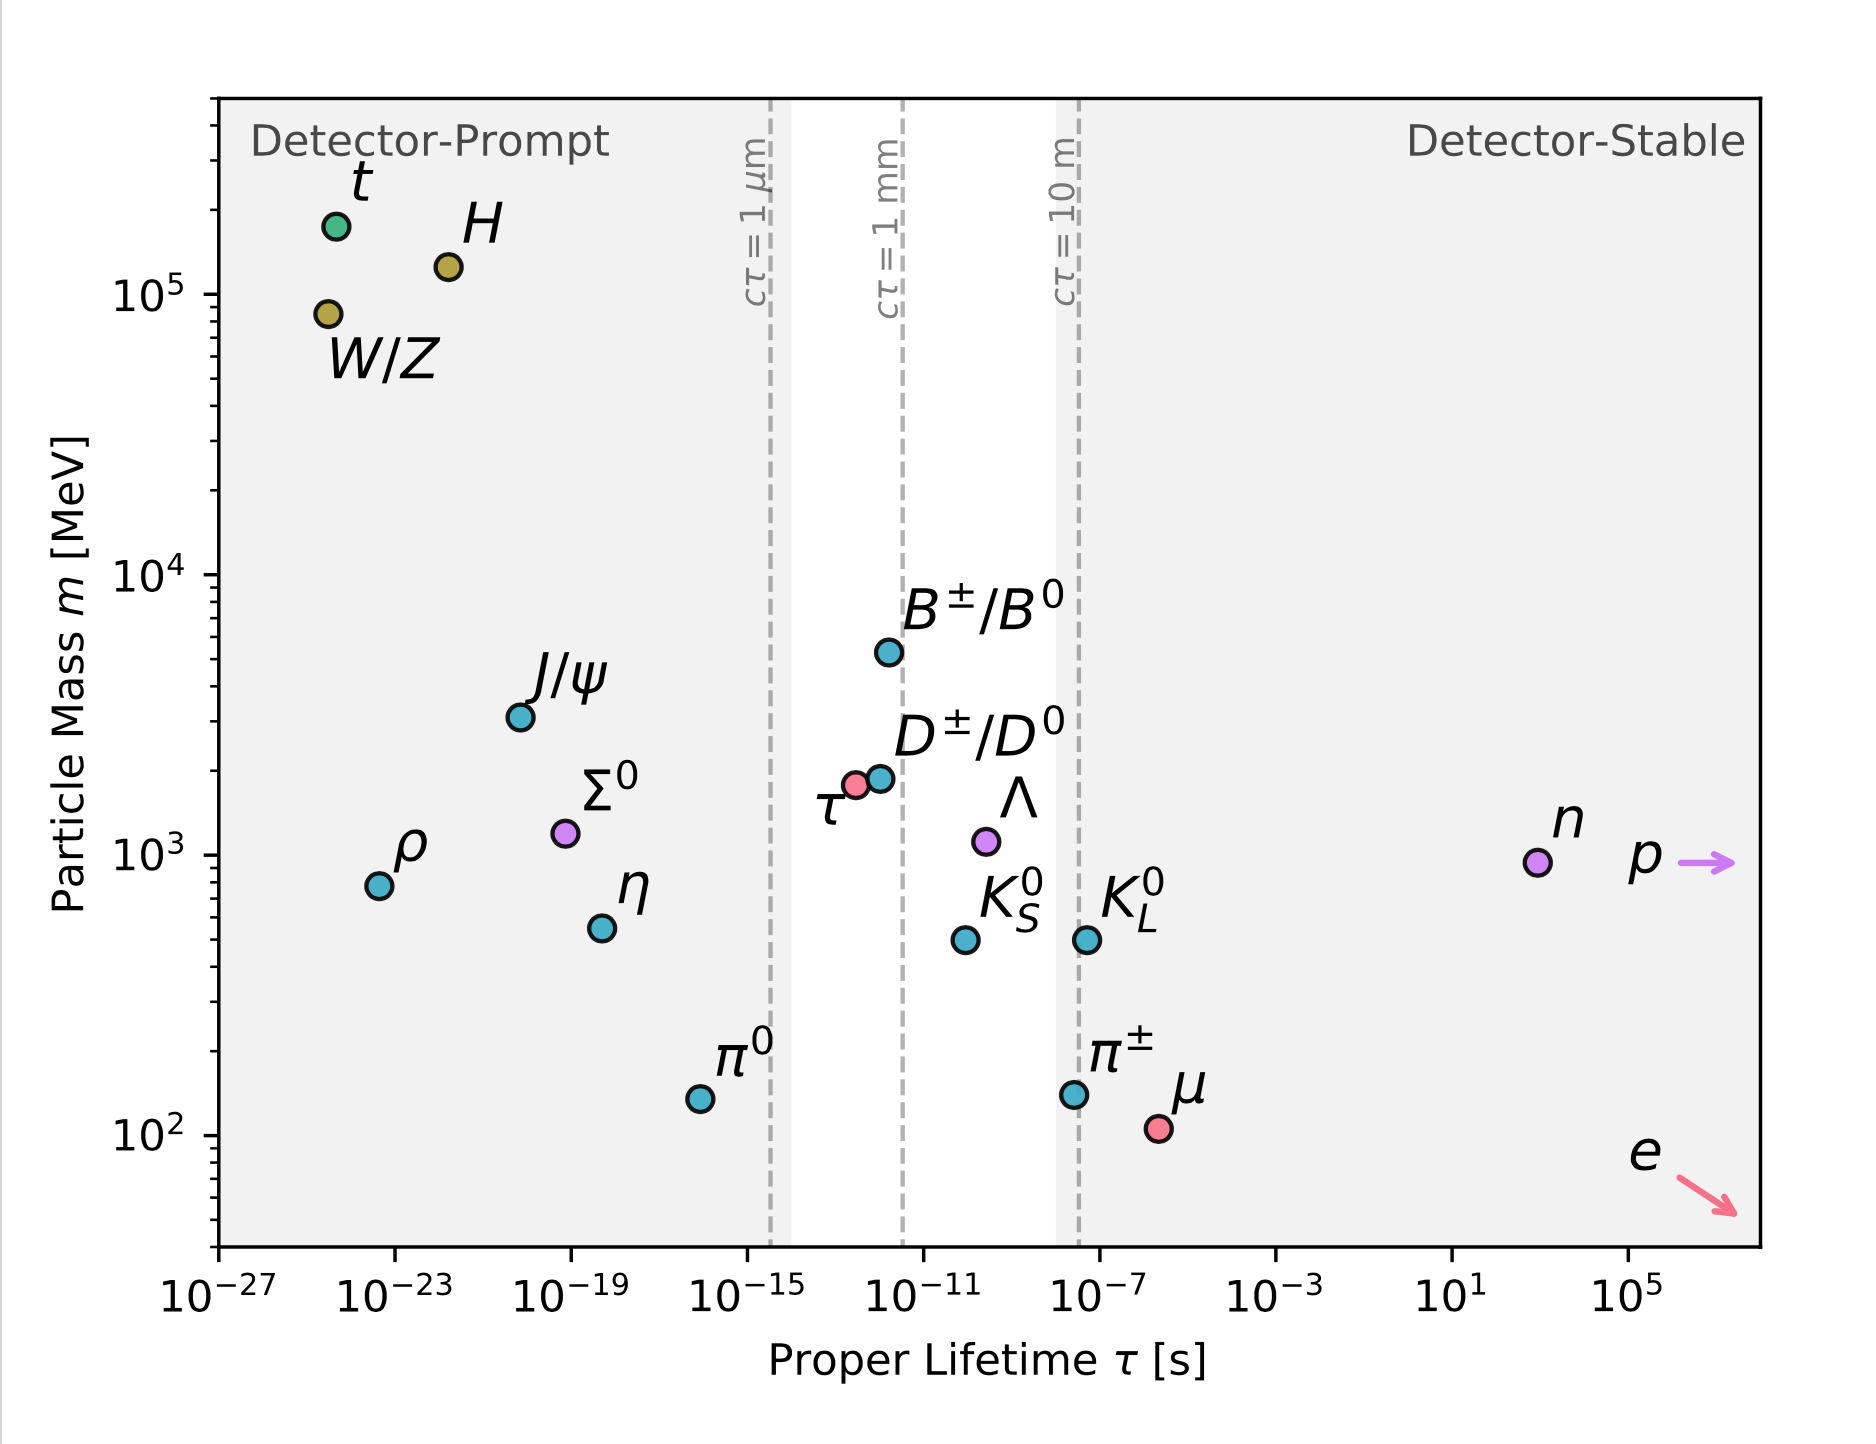
\includegraphics[width=.8\textwidth]{figures/theory/LLP-mass-lifetime.png}
\caption{A mass and proper lifetime distribution of particles in the \ac{SM}. There is a wide range of both masses and lifetimes. Shaded regions indicate detector-prompt or detector-stable particles. This assumes that particles traveling at the speed of light $\beta = 1$.}
\label{fig:trking_d0_eff}
\end{figure}


%other kinds of LLP signatures
